\documentclass[UTF8]{article}
\usepackage{ctex}
\usepackage{graphicx}
\usepackage{listings}
\begin{document}
    \section*{操作系统概述}
    为解决人机矛盾及CPU和I/O设备之间速度不匹配的矛盾\\
    脱机I/O:脱离主机的情况下进行\\
    联机I/O:在主机的直接控制下进行\\
    \\
    硬实时任务:系统必须满足任务对截止时间的要求\\
    软实时任务:也有一个截止时间,但不严格\\
    \\
    从交互性,及时性和可靠性,将分时系统和实时系统进行比较:\\
    交互性:实时信息处理系统虽然也具有交互性,但这里人与系统的交互仅限于访问系统中某些特定的专用服务程序。它不像分时系统那样能向终端用户提供数据处理和资源共享等服务。\\
    及时性:实时信息处理系统对实时性的要求与分时系统类似,都是以人所能接受的等待时间来确定的;而实时控制系统的及时性,则是以控 制对象所要求的开始截止时间或完成截止时间来确定的,一般为秒级到毫秒级,甚至有的要低于100微秒。\\
    可靠性:分时系统虽然也要求系统可靠,但相比之下,实时系统对可靠性的要求更高。因为任何差错都可能带来巨大的经济损失,甚至是无 法预料的灾难性后果,所以在实时系统中,往往都采取了多级容错措施来保障系统的安全性及数据的安全性。\\
    \\
    操作系统的特征:\\
    1.并发性:是指两个或多个事件在同一时间间隔内发生。\\
    2.共享性:是指系统中的资源可供内存中多个并发执行的进程(线程)共同使用,相应地,把这种资源的共同使用称为资源共享,或称为资源复用。\\
    3.虚拟性:是指通过某种技术把一个物理实体变为若干个逻辑上的对应物。\\
    4.异步性:进程是以人们不可预知的速度向前推进,即不确定性。其中,并发特征是操作系统最基本的特征,其它三个特征都是以并发特征为前提的。\\
    \\
    处理机管理的主要功能是:进程控制,进程同步,进程通信和调度\\
    1.进程控制:为作业创建进程,并为之分配必要的资源;进程结束时撤销进程,及时回收该进程所占用的各类资源;以及控制进程在运行过程中的状态转换;\\
    2.进程同步:为多个进程(线程)的运行进行协调,协调分为进程互斥方式和进程同步方式.\\
    3.进程通信:用来实现在相互合作的进程之间的信息交换;\\
    4.处理机调度:在后备队列上等待的每个作业都必须经过调度才能执行,在传统的操作系统中,
    包括作业调度和进程调度两步:\\
    (1)作业调度:从后备队里按照一定的算法,选择出若干个作业,为它们分配运行所需的资源(首先是分配内存).\\
    (2)进程调度:从进程的就绪队列中,按照一定算法选出一个进程,把处理机分配给它,并为它设置运行现场,使进程投入执行.\\
    \\
    内存管理的主要功能有:内存分配,内存保护,地址映射和内存扩充.\\
    1.内存分配:内存分配的主要任务是为每道程序分配内存空间,使它们"各得其所";
    提高存储器的利用率,减少不可用的内存空间;
    允许正在运行的程序申请附加的内存空间,以适应程序和数据动态增长的需要.\\
    2.内存保护:内存保护的主要任务是确保每道用户程序都只在自己的内存空间内运行,彼此互不干扰;
    决不允许用户程序访问操作系统的程序和数据;
    也不允许用户程序转移到非共享的其他用户程序中去执行.\\
    3.地址映射:为使程序能正确运行,存储器管理必须提供地址映射功能,以将地址空间中的逻辑地址转换为内存空间中与之对应的物理地址,
    该功能在硬件的支持下完成.\\
    4.内存扩充:借助于虚拟存储技术,从逻辑上去扩充内存容量,使用户所感觉的内存容量比实际内存容量大得多,
    以便让更多的用户程序并发运行.\\
    \\
    设备管理的主要功能有:缓冲管理,设备分配和设备处理.设备管理的主要任务是完成用户进程提出的I/O请求,为用户进程分配其所需的I/O设备;
    提高CPU 和I/O设备的利用率;
    提高I/O设备处理速度;方便用户使用I/O设备。\\
    1.缓冲管理:可有效地缓和CPU与I/O设备速度不匹配的矛盾,提高CPU的利用率,进而提高系统吞吐量;\\
    2.设备分配:设备分配的基本任务是根据用户进程的I/O请求、系统的现有资源情况以及按照某种设备的分配策略,为之分配其所需的设备;\\
    3.设备处理:设备处理程序又称为设备驱动程序。其基本任务是实现CPU和设备控制器之间的通信。\\
    \\
    文件管理主要功能有文件存储空间的管理、目录管理、文件的读/写管理和保护。文件管理的主要任务是对用户文件和系统文件进行管理,以方便用户使用,并保证文件的安全性。\\
    1.文件存储空间的管理:其主要任务是为每个文件分配必要的外存空间,提高外存的利用率,并能有助于提高文件系统的存、取速度。\\
    2.目录管理:目录管理的主要任务是为每个文件建立其目录项,并对众多的目录项加以有效的组织,以方便实现按名存取,即用户只须提供文件名便可对该文件进行存取。\\
    3.文件的读/写管理和保护:该功能是根据用户的请求,从外存中读取数据,或将数据写入外存,同时防止系统中的文件被非法窃取和破坏。\\
    \section*{进程管理}
    在操作系统中为什么要引入进程的概念?它会产生什么样的影响?\\
    在多道程序环境下,程序的执行属于并发执行,此时它们将失去其封闭性,并具有间断性及不可再现性的特征。这决定了通常的程序是不能参与并发执行的,因为程序执行的结果是不可再现的。这样,程序的运行也就失去了意义。为使程序能并发执行,且为了对并发执行的程序加以描述和控制,人们引入了“进程”的概念。传统0S中的进程定义为:“进程是进程实体的运行过程,是系统进行资源分配和调度的一个独立单位”,进程的引入使程序的并发执行得以实现.\\
    \\
    试说明PCB的作用,为什么说PCB是进程存在的惟一标志?\\
    进程控制块PCB(Process Control Block)是进程实体的一部分,是操作系统中最重要的记录型数据结构。PCB中记录了操作系统所需的、用于描述进程的当前情况以及控制进程运行的全部信息。进程控制块的作用是使一个在多道程序环境下不能独立运行的程序(含数据),成为一个能独立运行的基本单位,一个能与其它进程并发执行的进程。在进程的整个生命期中,系统总是通过PCB对进程进行控制,即系统是根据进程的PCB而非其他感知到该进程的存在的。所以说,PCB是进程存在的惟一标志。\\
    \\
    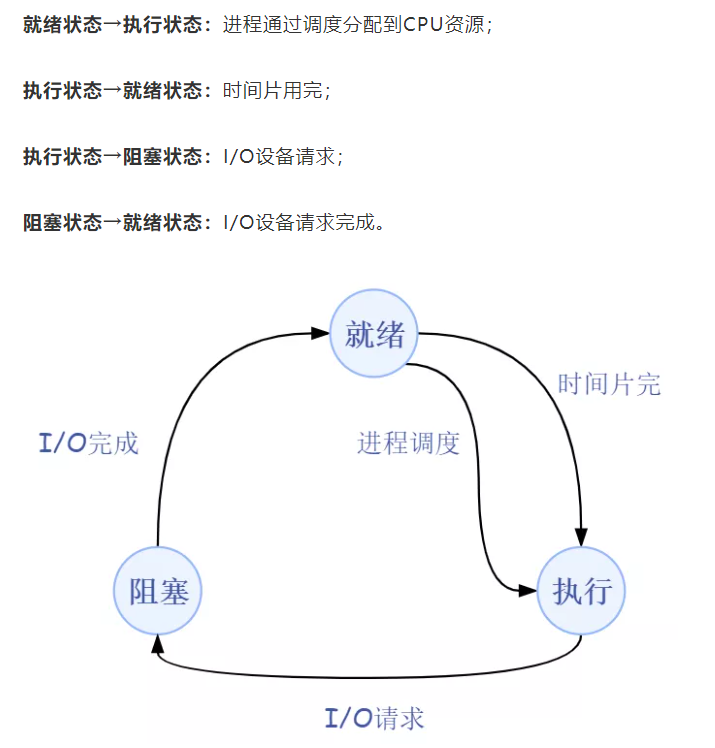
\includegraphics{graph/1.png}
    \\
    在创建一个进程时所要完成的主要工作是什么?\\
    一旦操作系统发现了要求创建新进程的事件后,便调用进程创建原语Creat()按下述步骤创建一个新进程:\\
    1.申请空白PCB:为新进程申请获得唯一的数字标识符,并从PCB集合中索取一个空白PCB.\\
    2.为新进程分配资源:为新进程的程序和数据以及用户栈分配必要的内存空间.\\
    3.初始化进程控制块:包括初始化标识信息,初始化处理机状态信息,初始化处理机控制信息.\\
    4.将新进程插入就绪队列,如果进程就绪队列能够接纳新进程,便将新进程插入就绪队列.\\
    \\
    \lstset{language=C}
    \begin{lstlisting}
        void P(S){//wait
            S.value=S.value-1;
            if(S.value<0){
                block(S,L);//加入阻塞队列
            }
        }

        void V(S){//signal
            S.value=S.value+1;
            if(S.value<=0){
                wakeup(L);//从阻塞队列中唤醒
            }
        }
    \end{lstlisting}
    高级调度又称为作业调度或长程调度,其主要功能是根据某种算法,把外存上处于后备队列中的那些作业调入内存,
    也就是说,它的调度对象是作业。\\
    低级调度用于决定就绪队列中的哪个进程(或内核级线程,为叙述方便,以后只写进程)应获得处理机,然后再由分派程序执行把处理机分配给该进程的具体操作。通常也把低级调度称为进程调度或短程调度,它所调度的对象是进程(或内核级线程)。 \\
    引入中级调度的主要目的是为了提高内存利用率和系统吞吐量。中级调度实际上就是存储器管理中的对换功能。\\
    \\
    为什么说多级反馈队列调度算法能较好地满足各方面用户的需要?\\
    1.终端型作业用户。由于终端型作业用户所提交的作业大多属于交互型作业,作业通常较小,系统只要能使这些作业(进程)在第一队列所规定的时间片内完成,便可使终端型作业用户都感到满意;\\
    2.短批处理作业用户。对于很短的批处理型作业,开始时像终端型作业一样,如果仅在第一队列中执行一个时间片即可完成,便可获得与终端型作业一样的响应时间。对于稍长的作业,通常也只需在第二队列和第三队列各执行一个时间片即可完成,其周转时间仍然较短;\\
    3.长批处理作业用户。对于长作业,它将依次在第1,2,…,n个队列中运行,然后再按轮转方式运行,用户不必担心其作业长期得不到处理。\\
    \\
    何谓死锁?产生死锁的原因和必要条件是什么?\\
    所谓死锁,是指多个进程在运行过程中因争夺资源而造成的一种僵局,当进程处于这种僵持状态时,若无外力作用,它们都将无法再向前推进。\\
    产生死锁的原因可归结为竞争资源引起进程死锁和进程推进顺序不当引起死锁两个方面。\\
    产生死锁的必要条件有互斥条件,请求和保持条件,不剥夺条件和环路等待条件。 \\
    \\
    在解决死锁问题的几个方法中,哪种方法最易于实现?哪种方法使资源利用率最高?\\
    为保证系统中诸进程的正常运行,应事先采取必要的措施,来预防发生死锁。在系统中已经出现死锁后,则应及时检测到死锁的发生,并采取适当措施来解除死锁。目前,处理死锁的方法可归结为以下四种:\\
    1.预防死锁\\
    摒弃请求和保持条件,摒弃不剥夺条件,摒弃环路等待条件\\
    2.避免死锁\\
    银行家算法\\
    3.检测死锁\\
    死锁定理\\
    4.解除死锁\\
    剥夺资源,撤销进程\\
    其中,预防死锁最容易实现,避免死锁使资源利用率最高
    \section*{内存管理}
    在理想情况下,存储器的速度应该非常快,能跟上处理机的速度,容量也非常大而且价格还应很便宜,但目前无法同时满足这样三个条件, 于是在现代计算机系统中,存储部件通常是采用层次结构来组织的。\\
    主要表现在:\\
    1.设置多个存储器可以使存储器两端的硬件能并行工作;\\
    2.采用多级存储系统,特别是Cache技术,是减轻存储器带宽对系统性能影响的最佳结构方案;\\
    3.在微处理机内部设置各种缓冲存储器,减轻对存储器存取的压力;\\
    4.增加CPU中寄存器数量能大大缓解对存储器的压力。\\
    \\
    1.绝对装入方式,只适用于单道程序环境。程序中适用绝对地址,程序中的逻辑地址与实际内存地址完全相同。绝对装入方式只能将目标模块装入到内存中事先指定的位置。适用的场合:绝对装入方式只适用于单道程序环境,而且必须事先已知用户程序(进程)驻留在内存开始位置R,则编译程序所产生的目标模块(即装入模块)便从R处开始向上扩展;\\
    2.可重定位装入方式,适用于多道程序环境,但不允许程序运行时在内存中移动位置,在程序装入时一次性完成地址变换。在采用可重定位装入程序将装入模块装入内存后,会使装入模块中的所有逻辑地址与实际装入内存的物理地址不同。适用的场合:可重定位装入方式可将装入模块装入到内存中任何允许的位置,故可用于多道程序环境,但这种方式并不允许程序运行时在内存中移动位置;\\
    3.动态运行时装入方式,用于多道程序环境,动态运行时的装入程序在把装入模块装入内存后,并不立即把装入模块中的相对地址转换为绝对地址,而是把这种地址转换推迟到程序真正要执行时才进行。因此,装入内存后的所有地址都仍是相对地址。适用场合:在程序运行过程中它在内存中的位置经常要改变的情况下,只能选择动态运行时装入方式.\\
    \\
    1.静态链接:在程序运行之前,先将各目标模块及它们所需的库函数,链接成一个完整的装配模块,以后不再拆开。我们把这种事先进行链接的方式称为静态链接方式;\\
    2.装入时动态链接:是指用户源程序经编译后所得的目标模块,是在装入内存时边装入边链接的,即在装入一个目标模块时,若发生一个外部模块调用事件,将引起装入程序去找出相应的外部目标模块,并将它装入内存。优点是:便于修改和更新;便于实现对目标模块的共享;\\
    3.运行时动态链接:是对装入时动态链接方式的一种改进,是指对某些目标模块的链接,是在程序执行中需要该目标模块时,才对它进行链接的链接方式。对某些模块的链接推迟到程序执行时才进行链接,亦即,在执行过程中,当发现一个被调用模块尚未装入内存时,立即由OS去找到该模块并将之装入内存,把它链接到调用者模块上。凡在执行过程中未被用到的目标模块,都不会被调入内存和被链接到装入模块上,这样不仅可加快程序的装入过程,而且可节省大量的内存空间。\\
    \\
    引入分段存储管理方式,主要是为了满足用户和程序员的下述一系列需要:\\
    1.方便编程。用户把自己的作业按照逻辑关系划分为若干个段,每个段都从0开始编址,并有自己的名字和长度。因此,希望访问的逻辑地址是由段名(段号)和段内偏移量(段内地址)决定的;\\
    2.信息共享。在实现对程序和数据的共享时,是以信息的逻辑单位为基础的。分页系统中的页是存放信息的物理单位,并无完整意义,不便于共享;然而段是信息的逻辑单位。由此可见,为了实现段的共享,希望存储管理能与用户程序分段的组织方式相适应;\\
    3.信息保护。信息保护同样对信息的逻辑单位进行保护,因此,分段管理方式能更有效和更方便地实现信息保护功能;\\
    4.动态增长。在实际应用中,往往有些段特别是数据段,在使用过程中会不断地增长,而事先无法确切地知道会增长到多大,而分段存储管理方式能较好地解决这一问题;\\
    5.动态链接。动态链接是指在作业运行之前,并不把目标程序段链接起来。要运行时,先将主程序所对应的目标程序装入内存并启动运行,当运行过程中又需要调用某段时,才将该段(目标程序)调入内存并进行链接。可见动态链接也要求以段作为管理的单位。\\
    \\
    为什么说分段系统比分页系统更易于实现信息的共享和保护?\\
    1.分页系统中的每个页面是分散存储的,为了实现信息共享和保护,页面之间需要一一对应,为此需要建立大量的页表项;\\
    2.分段系统中的每个段都从0编址,并采用一段连续的地址空间,在实现共享和保护时,只需为要共享和保护的程序设置一个段表项,将其中的基址与内存地址一一对应就能实现信息的共享和保护。\\
    \\
    分段和分页存储管理的区别主要表现在:\\
    1.页是信息的物理单位,分页是为实现离散分配方式,以消减内存的外零头,提高内存利用率。或者说,分页仅仅是由于系统管理的需要而不是用户的需要。段则是信息的逻辑单位,它含有一组意义相对完整的信息,分段的目的是为了能更好地满足用户的需要;\\
    2.页的大小固定且由系统决定,由系统把逻辑地址划分为页号和页内地址两部分,是机械硬件实现的,因而在系统中只能有一种大小的的页面;而段的长度却不固定,决定于用户所编写的程序,通常由编译程序对源程序进行编译时,根据信息的性质来划分;\\
    3.分页的作业地址空间是一维的,即单一的线性地址空间,程序员只需利用一个记忆符,即可表示一个地址;分段的作业地址空间则是二维的,程序员在标识一个地址时,既需给出段名,又需给出段内地址。\\
    \\
    在请求分页系统中,页表应包括哪些数据项?每项的作用是什么?\\
    页表应包括页号、物理块号、状态位P、访问字段A、修改位M和外存地址。现对其中各数据项说明如下:\\
    1.状态位P:用于指示该页是否已调入内存,供程序访问时参考;\\
    2.访问字段A:用于记录本页在一段时间内被访问的次数,或记录本页最近已有多长时间未被访问,供选择换出页面时参考;\\
    3.修改位M:表示该页在调入内存后是否被修改过。由于内存中的每一页都在外存上保留一份副本,因此,若未被修改,在置换该页时就不需再将该页写回到外存上,以减少系统的开销和启动磁盘的次数;若已被修改,则必须将该页重写到外存上,以保证外存中所保留的始终是最新副本。简言之,M位供置换页面时参考;\\
    4.外存地址:用于指出该页在外存上的地址,通常是物理块号,供调入该页时参考\\
    \section*{文件管理}
    顺序文件的结构可以归纳为两种情况:\\
    1.串结构,各记录之间的顺序与关键字无关,通常的办法是由时间来决定,即按存入时间的先后排列,最先存入的记录作为第一个记录,其次存入的为第二个记录……,依此类推;\\
    2.顺序结构,文件中的所有记录按关键字(词)排列,可以按关键词长短排序或按英文字母顺序排序。顺序文件的最佳应用场合是对诸记录进行批量存取时,即每次要读或写一大批记录时。\\
    \\
    索引文件是为可变长记录文件建立一张索引表,对主文件中的每个记录在索引表中设有一个相应的表项,用于记录该记录的长度L及指向该记录的指针(指向该记录在逻辑地址空间的首址),以加快对记录检索的速度。\\
    引入多级索引:为了进一步提高检索速度,使用户的访问速度更快,引入了多级索引结构,它可以有效地管理索引文件,根据用户的访问情况进行多级处理。\\
    \\
    
\end{document}